\section*{Effetto dell'esposizione a \emph{$CdCl_{2}$} e MMR di mutanti al sistema di riparazione dei mal appaiamenti "Mismatch Repair"}

	\subsection*{Introduzione}
	Questo esperimento valuterà la qualità della trasmissione del DNA, ma concentrandosi sui meccanismi di riparazione dello stesso in diverse condizioni ambientali, piuttosto che prendere ad esempio la sola replicazione, come nelle esperienze precedenti. 
	Si cercherà di comprendere le eventuali esposizioni ambientali su di un gene e la bontà della replicazione del DNA, focalizzandosi su errori di replicazione che vengono - o non vengono - riparati. 

 
	\subsubsection*{I genotipi dei ceppi}
	Può succedere in vivo che una polimerasi catalizzi il nucleotide sbagliato durante il processo di replicazione, ma questo errore può essere ancora riconosciuto e risolto. 
	I due modi in cui una cellula ripara i \emph{mismatch} sono l'attività di proofreading polimerasica ed il sistema di riparazione dei mal appaiamenti (MMR). 
	Volendo studiare mutazioni causate da mismatch, a questo punto sorge un'ambiguità: la mutazione potrebbe essere stata causata dal fallimento dell'attività esonucleasica della polimerasi, da un errore nel nucleotide incorporato erroneamente o del DNA \emph{mismatch repair} (MMR). 
	Si è costruito un sistema che permettesse di superare l'ambiguità causata da questa doppia linea di difesa contro i mal appaiamenti. 
	Si è visto che in lunghe sequenze omonucleotidiche la polimerasi tende ad introdurre un nucleotide in più. 
	Se la sequenza omonucleotidica da copiare è ricca soprattutto in A e T e diventa lunga, precisamente maggiore di 7, la correzione di bozze sembra essere totalmente inefficace. 
	Rimane quindi un solo meccanismo di riparazione, MMR appunto, ed è su questa osservazione che si basa il nostro esperimento. 
	Non tutte le sequenze di DNA sono replicabili con la stessa efficacia, quelle che potrebbero rappresentare siti di mutazione vengono chiamate \emph{at risk motifs}. 
	Vogliamo testare, sfruttando queste sequenze più fragili, se alcune condizioni nel terreno, come agenti mutageni, possono interferire con il sistema MMR. 
	La sostanza mutagena scelta è il cadmio cloruro (CdCl$_{2}$). 
	In vivo si ha bisogno di un saggio reporter, nel nostro caso un gene importante nella biosintesi della lisina, il gene \emph{LYS2}. 
	Si ha a disposizione un ceppo il quale è stato precedentemente sottoposto ad un intervento di ingegnerizzazione, nel quale il gene \emph{LYS2} è stato inattivato da uno \emph{stretch} omonucleotidico di 14 A. 
	Il quadro di lettura del nostro ceppo sarà quindi sfalsato a valle a causa delle 13 adenine esogene, inserite per altro al centro della sequenza codificante, impedendo al ceppo di vivere in un terreno senza lisina. 
	Oltre al ceppo che in questo esperimento chiamiamo \emph{wild type} (WT), si sono sfruttati altri tre ceppi: $\delta$msh2, nel quale è stato inattivato il gene \emph{msh2}, $\delta$msh6 nel quale è stato reso inattivo il gene \emph{mlh1} ed infine, $\delta$msh6, con gene \emph{msh6} spento. 
	Questi tre geni silenziati codificano ciascuno per una proteina che fa parte del complesso proteico coinvolto del sistema di riparazione dei mismatch. 
	Di seguito si riportano i genotipi. 
	\begin{itemize}
		\item WT\emph{(MATalpha, ade5-1 his 7-2 leu 2-3, 112 trp1-289 ura3-52 lys2::insE-A14)}.
		\item $\delta$msh2(isogenico al WT tranne per la \emph{msh2::kanMX}).
		\item $\delta$mlh1(isogenico al WT tranne per la \emph{mlh1::kanMX}).
		\item $\delta$msh6(isogenico al WT tranne per la \emph{msh6::kanMX}).
	\end{itemize}
 
 
\subsubsection*{Preparazione dell'esperimento}
La preparazione all'esperimento si è svolto nell'arco dei tre giorni. 
Per prima cosa, partendo dalle colonie di ciascun ceppo di lievito fornite, si sono preparate due \emph{patches} su una piastra YPDA, seguendo lo schema riportato sul protocollo, usando stecchi sterili. 
Si è lasciato incubare a 30 C° durante la notte. 
Il giorno dopo le piastre con i \emph{patches} di ceppi mutanti sono state replicate su cinque diverse piastre con la tecnica di replica plating, usando un panno di velluto. 
Una piastra contiene un terreno SD complete, da usare come controllo; un'altra con SD lys, deficiente di lisina; altre due piastre SD lys CdCl$_{2}$, rispettivamente con una dose di cadmio cloruro di 0.5
$\mu$M e 5$\mu$M; un'ultima piastra contente SD his, un terreno privo di istidina. 
Si sono lasciate queste piastre ad incubare a 30 C° e quattro giorni dopo si è potuto apprezzare il risultato.
 
\subsection*{Risultati ottenuti}
Come ci si aspettava, nella piastra contenente un media completo (figura~\ref{fig5})
tutti i diversi ceppi sono cresciuti senza rilevazione di sostanziali differenze. 
Nella piastra con terreno senza lisina (figura~\ref{fig6})
possiamo invece osservare che il ceppo WT non è riuscito a crescere, con apparizione di 17 colonie totali. 
I ceppi $\delta$msh2 e $\delta$mlh1 hanno visto una crescita importante, mentre il ceppo $\delta$msh6 leggermente minore alle due precedenti. 
Un risultato molto simile, con una differenza di quantità di colonie sostanziale solo per WT, è stata registrata per la piastra con una dose di cadmio cloruro pari a 0,5$\mu$M (figura~\ref{fig2}) e per quella contente 5$\mu$M di CdCl$_{2}$.
Una differenza visibile tra le due piastre contenenti CdCl$_{2}$ e quella SD lys è che le colonie nelle prime due sono leggermente più piccole, anche se in numero maggiore, circa il doppio. 
Diversamente dalle altre, la piastra in cui era assente l'istidina, ha visto una crescita minima di tutti di ceppi: crescita nulla per WT, appena una 20ina di colonie per \emph{patch} per i ceppi $\delta$msh2 e $\delta$mlh1. 
Si osservano ora colonie di ceppi mutanti cresciuti su terreni diversi.
\begin{multicols}{3}
	
	\begin{figure}[H]
		\centering
		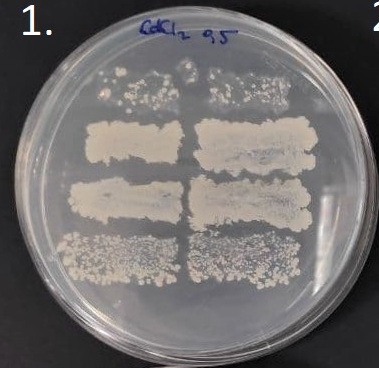
\includegraphics[scale=0.4]{./Pics/GeniAmbiente/CdCl05.jpg}
		\caption{Terreno con \emph{$CdCl_2$} $0.5\si{\micro M}$ e deficiente di lisina}
		\label{fig2}
	\end{figure}

	\begin{figure}[H]
		\centering
		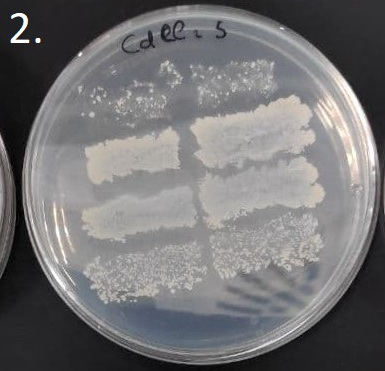
\includegraphics[scale=0.4]{./Pics/GeniAmbiente/CdCl5.jpg}
		\caption{Terreno con \emph{$CdCl_2$} $5\si{\micro M}$ e deficiente di lisina}
		\label{fig3}
	\end{figure}

	\begin{figure}[H]
		\centering
		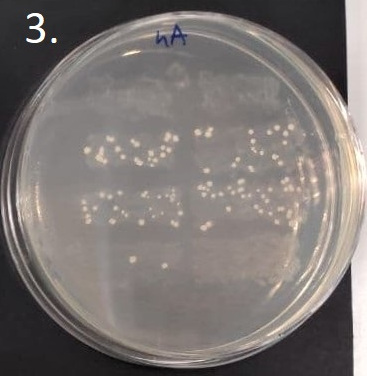
\includegraphics[scale=0.4]{./Pics/GeniAmbiente/hA.jpg}
		\caption{Terreno deficiente di istidina}
		\label{fig4}
	\end{figure}

	\begin{figure}[H]
		\centering
		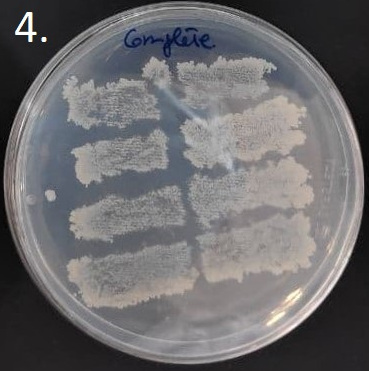
\includegraphics[scale=0.4]{./Pics/GeniAmbiente/Complete.jpg}
		\caption{Terreno completo}
		\label{fig5}
	\end{figure}

	\begin{figure}[H]
		\centering
		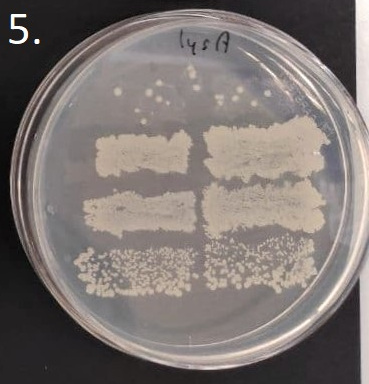
\includegraphics[scale=0.4]{./Pics/GeniAmbiente/lysA.jpg}
		\caption{Terreno deficiente di lisina}
		\label{fig6}
	\end{figure}

\end{multicols}
 
 
\subsection*{Conclusioni}
La quantificazione della reversione del gene \emph{LYS2} consente di stimare il numero di mal appaiamenti risolti grazie a MMR. 
Il ceppo nella prima linea di ogni piastra è il ceppo WT, di cui si è discusso ampiamente all'inizio di questa sezione. 
Il motivo per cui WT non riesce a crescere in un terreno privo di lisina è lo shift del quadro di lettura causato dall'inserimento di 13 adenine. 
Se però ci fosse un errore di sintesi del DNA, nella quale la polimerasi lascia indietro una adenina, si avrebbe una discendenza nella quale le cellule hanno 12 adenine esogene, restaurando il quadro di lettura mantenendo le stesse triplette in tutto il genoma a valle dell'inserzione e il mutante tornerebbe a crescere in un terreno senza lisina. 
Questo effetto lo si vede in ogni piastra nella prima riga con l'apparizione di colonie revertanti. 
Affinché la cellula si "lasci sfuggire" un nucleotide, MMR deve commettere un errore. 
Ciò spiega perchè nelle piastre in cui è presente il cadmio cloruro si vedono più colonie revertanti del ceppo WT: essendo le colonie raddoppiate in piastre contenenti il mutageno, si può affermare che il sistema di MMR è stato compromesso dal cadmio cloruro, permettendogli di fare più errori e permettere una crescita maggiore. 
Per quanto riguarda gli altri ceppi, la differenza non è così sostanziale perchè il loro MMR era già compromesso. 
Possono nascere altre considerazioni da questi risultati. 
Uno riguarda sicuramente i mutanti $\delta$msh6. 
Il tasso di reversione è minore rispetto agli altri due ceppi mutanti perchè la proteina codificata dal gene silenziato non riveste un ruolo di fondamentale importanza nell'economia del sistema di MMR, facendo parte di un eterodimero facoltativo con la proteina MSH2. 
MSH2 infatti può dimerizzare sia con MSH6, che con MSH3, non rendendo così vitale la funzione di MSH6. 
Un'altra osservazione può essere condotta sulla differenza non presente tra le due piastre con concentrazione presente di CdCl$_{2}$. 
Perchè nella piastra con concentrazione di 5$\mu$M non si è vista una crescita molto maggiore? Con ogni probabilità, il CdCl$_{2}$ ad una concentrazione così alta supera una soglia di tossicità che impedisce la proliferazione cellulare. 
Non solo, un piccolo ruolo potrebbe essere rivestito anche dalla tecnica di replica plating: le piastre replicate per ultime potrebbero contenere in partenza un minor nuemero di cellule di lievito. 
Le ultime parole potrebbero essere spese per la piastra contenente SD hisA, cioè media sintetico senza istidina. 
C'è una bassa crescita cellulare perchè i ceppi sono auxotrofi, tra le varie cose, anche per l'istidina. 
Si può considerare questa piastrazione come un'ulteriore controllo riguardo la nostra sicurezza di stare considerando solo i meccanismi di mismatch repair. 
Il gene \emph{his} non è stato inattivato inserendo nella sequenza codificante un lungo stretch omonucleotidico come emph{lys2} e in questo caso l'attività di proofreading compie il lavoro di prima difesa contro gli errori di replicazione. 
Anche in questo caso però possiamo osservare come sia il MMR a fare la differenza in termini stocastici: nei ceppi in cui il MMR è inbito si può apprezzare una crescita cellulare di colonie revertanti. 
